% !TEX encoding = UTF-8 Unicode
%!TEX root = thesis.tex
% !TEX spellcheck = en-US
%%=========================================


\chapter{User manual}
The core functionality of the system is to create and view articles. All main functionality is accessible through the main menu on top of the screen. 


%% #################  Article  ##################
\section{Creating an article}
\paragraph{Step 1:} In order to create an article, you will need to go to the editor page. Click the editor button as marked in \ref{fig:manual1}. If you are signed in and authorised, go to step 3, if not, continue to step 2.

\begin{figure}[H]
    \centering
    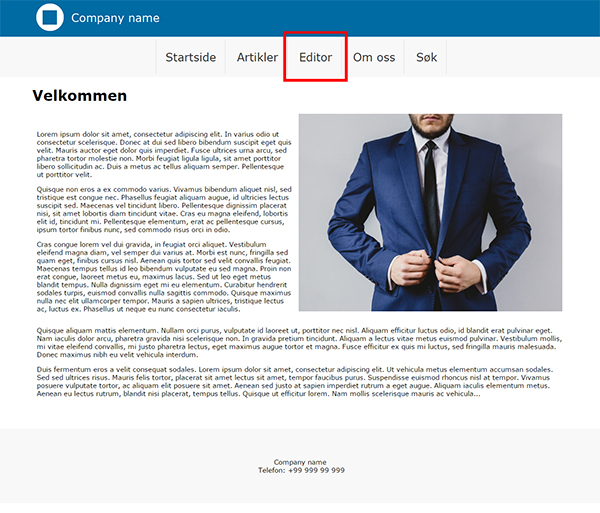
\includegraphics[scale=0.70]{fig/userManual/1}
    \caption{Showing location of the editor button in main menu}
    \label{fig:manual1}
\end{figure}


\paragraph{Step 2:} Fill in your credentials and log in as shown in figure \ref{fig:manual2}. This will prompt you with an authorisation screen. Click "Authorize" in order to get access (displayed in figure \ref{fig:manual3}).

\begin{figure}[H]
    \centering
    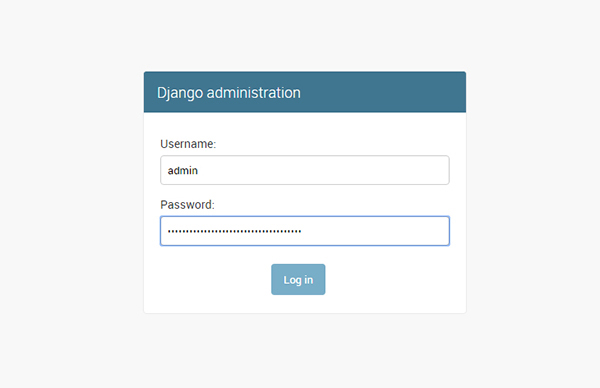
\includegraphics[scale=0.70]{fig/userManual/2}
    \caption{View for step 2}
    \label{fig:manual2}
\end{figure}

\begin{figure}[H]
    \centering
    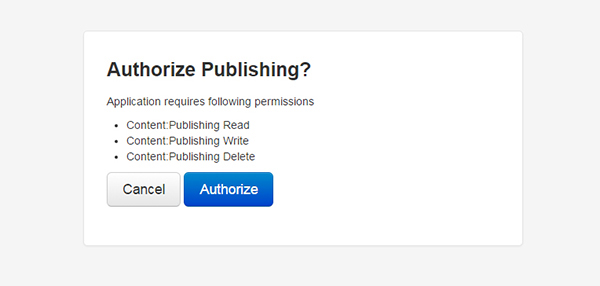
\includegraphics[scale=0.70]{fig/userManual/3}
    \caption{View for step 2}
    \label{fig:manual3}
\end{figure}

\paragraph{Step 3:} You will then need to choose which template you want to base your article on from the drop down list titled "Velg en mal".

\begin{figure}[H]
    \centering
    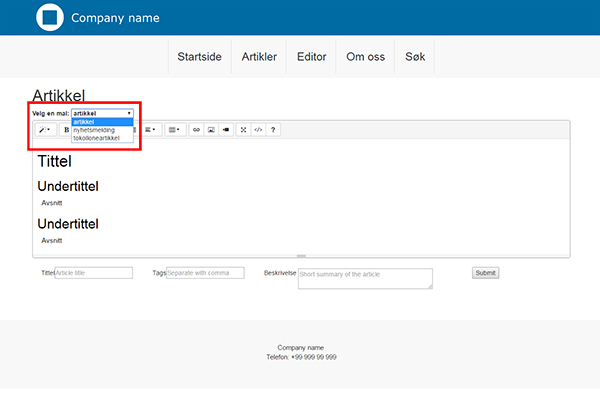
\includegraphics[scale=0.70]{fig/userManual/4}
    \caption{Showing location of the template drop-down list}
    \label{fig:manual4}
\end{figure}


\paragraph{Step 4:} Once you are done writing the article and adding metadata like title and description, you submit it by clicking the "submit"-button in the bottom-right corner. 
\begin{figure}[H]
    \centering
    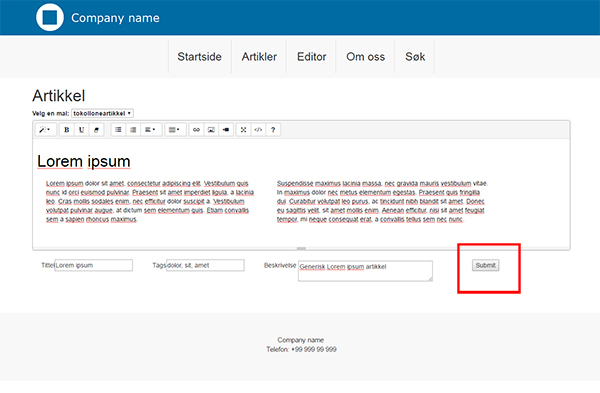
\includegraphics[scale=0.70]{fig/userManual/5}
    \caption{Showing location of the submit button}
    \label{fig:manual5}
\end{figure}


%% #################  Search  ##################
\section{Searching}
Articles can be found in two ways; either by finding them in the article list, as shown in figure \ref{fig:manual6}, or by searching. The following steps explain how to use the search function.

\begin{figure}[H]
    \centering
    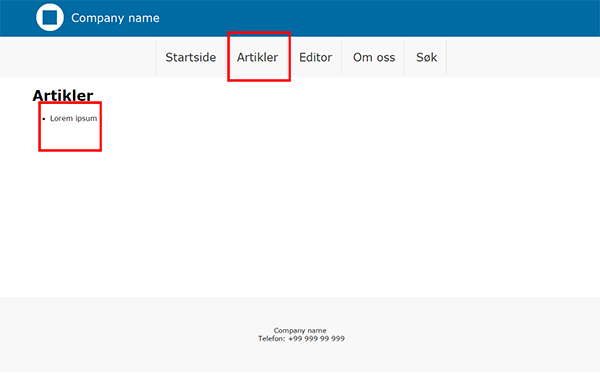
\includegraphics[scale=0.70]{fig/userManual/6}
    \caption{Showing location of the submit button}
    \label{fig:manual6}
\end{figure}

\paragraph{Step 1:} First, go to the search page as show in figure \ref{fig:manual7}.

\begin{figure}[H]
    \centering
    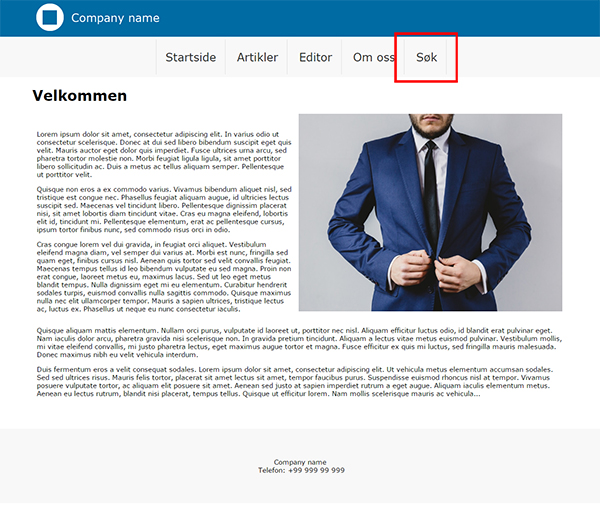
\includegraphics[scale=0.70]{fig/userManual/7}
    \caption{Showing location of the search button in main menu}
    \label{fig:manual7}
\end{figure}


\paragraph{Step 2:} When you start writing in the search field, it will give you suggestions of completions for potentially incomplete words. In order to accept this suggestion you can either left-click it or press the down-arrow on your keyboard. 

\begin{figure}[H]
    \centering
    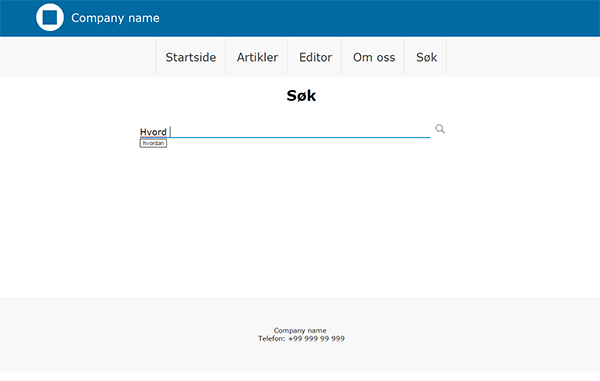
\includegraphics[scale=0.70]{fig/userManual/8}
    \caption{Word completion suggestion}
    \label{fig:manual8}
\end{figure}

\paragraph{Step 3:} Once your query is completed, you can search by either clicking the search icon or pressing the return key on your keyboard. This will present you with a suggestion to spelling in your query, which can be accepted the same way as suggestions in step 2. It will also present you with potential results, as shown in figure \ref{fig:manual9}.

\begin{figure}[H]
    \centering
    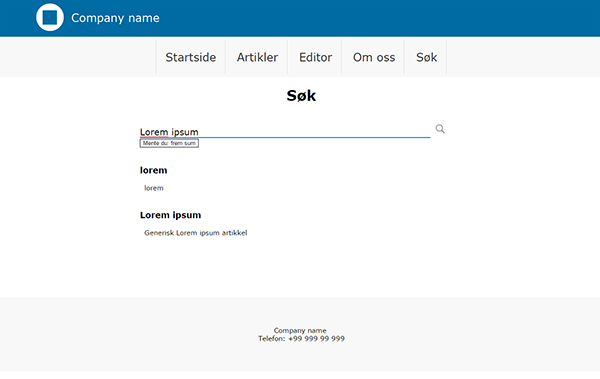
\includegraphics[scale=0.70]{fig/userManual/9}
    \caption{Search results}
    \label{fig:manual9}
\end{figure}

\paragraph{Step 4:} By clicking the article title you are brought to the full article as shown in figure \ref{fig:manual10}

\begin{figure}[H]
    \centering
    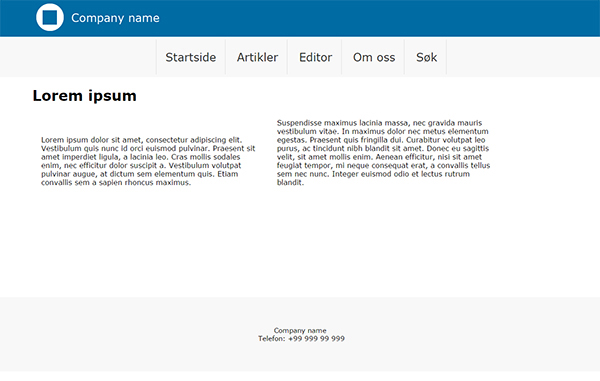
\includegraphics[scale=0.70]{fig/userManual/10}
    \caption{Full article}
    \label{fig:manual10}
\end{figure}




%% #################  Status  ##################
\section{Viewing service status}

\paragraph{Step 1:} Seeing as status is a developer feature, it is not clearly indicated with a button. In order to access it you need to click "Om oss" in the menu and then "Service status overview", as shown in figure \ref{fig:manual14}.

\begin{figure}[H]
    \centering
    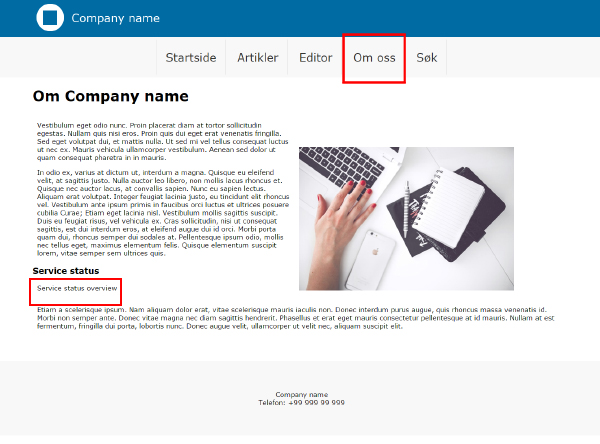
\includegraphics[scale=0.70]{fig/userManual/14}
    \caption{Hidden status button}
    \label{fig:manual14}
\end{figure}

\paragraph{Step 2:} By clicking 'show' on any of the services, you are provided extra information about its status. An example of the view for the indexer service can be seen in figure \ref{fig:manual11}.

\begin{figure}[H]
    \centering
    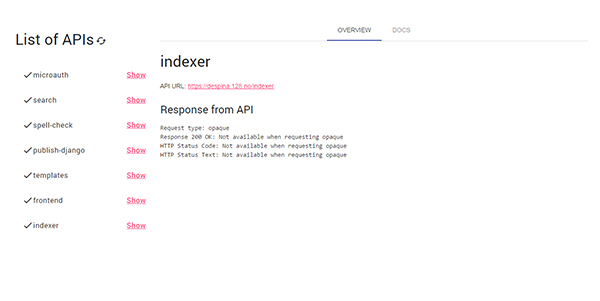
\includegraphics[scale=0.70]{fig/userManual/11}
    \caption{Status overview. The symbol in front of the name represents its state. Check mark means available and an error symbol means it's unavailable.}
    \label{fig:manual11}
\end{figure}
% The status of each service is indicated by a symbol in front of its name. A check mark indicates that its running, a spinner shows when it is querying the service and an error symbol when it's unavailable. 

\paragraph{Step 3:} For viewing the documentation for the service, click on "Docs" in the upper-right corner as highlighted in figure \ref{fig:manual12}.

\begin{figure}[H]
    \centering
    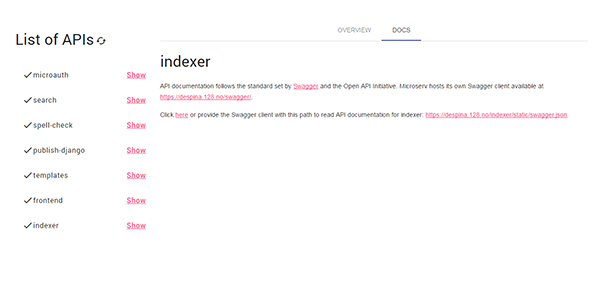
\includegraphics[scale=0.70]{fig/userManual/12}
    \caption{Service documentation}
    \label{fig:manual12} 
\end{figure}
